\section{Prueba}
Para comprobar el funcionamiento del proyecto, se realizo la siguiente grabación, la cual contiene una pequeña parte del Himno a la Alegría. Cuyas notas (de ese fragmento) son:\\
si4-si4-do5-re5-re5-do5\\
si4-la4-sol4-sol4-la4-si4-si4-la4-la4\\
si4-si4-do5-re5-re5-do5\\
El archivo wav con la grabación se aprecia en la Figura 4:
\begin{figure}[H]
	\begin{center}
		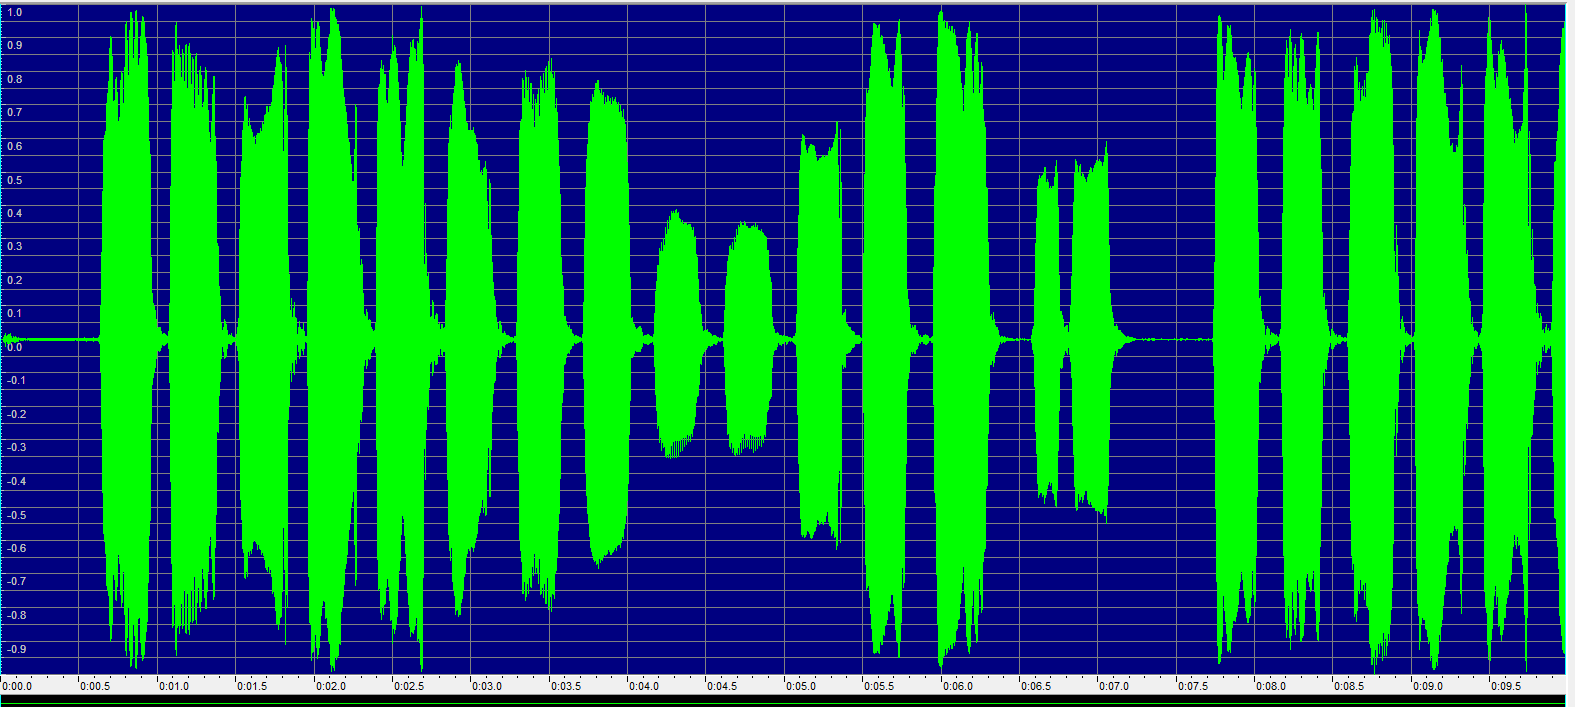
\includegraphics[scale=.35]{img/wav.png}
		\caption{Wav generado por la grabación-Contiene un fragmento del Himno a la Alegría}
		\label{fig:wav}
	\end{center}
\end{figure}
Al ingresar esta grabación al programa desarrollado, se obtuvo la siguiente salida:
\begin{figure}[H]
	\begin{center}
		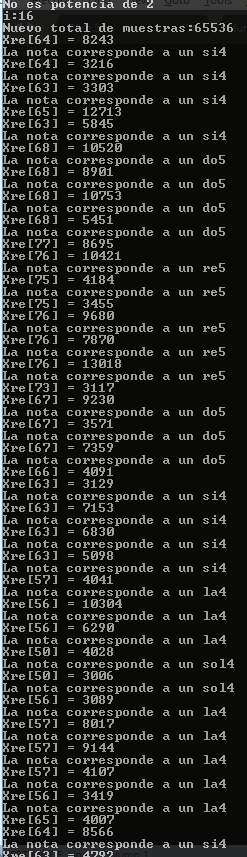
\includegraphics[scale=1]{img/salida1.png}
		\label{fig:wav1}
	\end{center}
\end{figure}
\begin{figure}[H]
	\begin{center}
		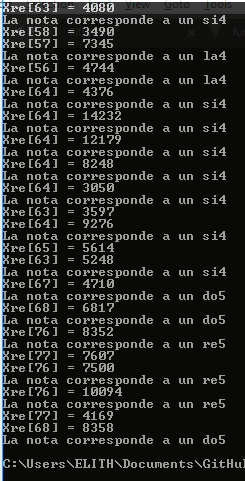
\includegraphics[scale=1]{img/salida2.png}
		\label{fig:wav1}
	\end{center}
\end{figure}